% PARTE 3: EJERCICIOS PROPUESTOS Y SOLUCIONES

\section{Ejercicios Propuestos}

\begin{nota}
Te recomendamos intentar resolver estos ejercicios por tu cuenta antes de ver las soluciones. ¡La práctica hace al maestro! Recuerda que las funciones inversas te dan el ángulo cuando conoces el valor de la función.
\end{nota}

\begin{ejercicio}
\textbf{Ejercicio 1 (Nivel Básico):} Calcula los siguientes valores exactos sin usar calculadora:

\begin{enumerate}[label=\alph*)]
\item $\arcsen(0)$
\item $\arccos(1)$
\item $\arctan(\sqrt{3})$
\item $\arcsen(-1)$
\item $\arccos(0)$
\item $\arctan(0)$
\end{enumerate}
\end{ejercicio}

\begin{ejercicio}
\textbf{Ejercicio 2 (Nivel Básico):} Determina el valor exacto de:

\begin{enumerate}[label=\alph*)]
\item $\arccos\left(\frac{\sqrt{2}}{2}\right)$
\item $\arcsen\left(-\frac{1}{2}\right)$
\item $\arctan(1)$
\item $\arcsen\left(\frac{\sqrt{3}}{2}\right)$
\item $\arccos\left(-\frac{1}{2}\right)$
\end{enumerate}
\end{ejercicio}

\begin{ejercicio}
\textbf{Ejercicio 3 (Nivel Intermedio):} Calcula sin usar calculadora:

\begin{enumerate}[label=\alph*)]
\item $\sen\left(\arccos\left(\frac{3}{5}\right)\right)$
\item $\cos\left(\arcsen\left(\frac{5}{13}\right)\right)$
\item $\tan\left(\arcsen\left(\frac{2}{3}\right)\right)$
\item $\sec\left(\arctan\left(\frac{4}{3}\right)\right)$
\end{enumerate}

\textit{Sugerencia: Usa triángulos rectángulos. Dibuja uno y asigna los lados según la información dada.}
\end{ejercicio}

\begin{ejercicio}
\textbf{Ejercicio 4 (Nivel Intermedio):} Simplifica las siguientes expresiones:

\begin{enumerate}[label=\alph*)]
\item $\sen(\arcsen(x))$ donde $-1 \leq x \leq 1$
\item $\arcsen(\sen(x))$ para $x \in [-\pi/2, \pi/2]$
\item $\tan(\arccos(x))$ donde $-1 \leq x \leq 1, x \neq 0$
\item $\cos(\arctan(x))$ para cualquier $x$ real
\end{enumerate}
\end{ejercicio}

\begin{ejercicio}
\textbf{Ejercicio 5 (Nivel Avanzado):} Resuelve las siguientes ecuaciones:

\begin{enumerate}[label=\alph*)]
\item $\arcsen(x) = \frac{\pi}{6}$
\item $\arccos(2x-1) = \frac{\pi}{3}$
\item $\arctan(x+1) = \frac{\pi}{4}$
\item $2\arcsen(x) = \frac{\pi}{2}$
\item $\arccos(x) + \arcsen(x) = \frac{\pi}{2}$
\end{enumerate}
\end{ejercicio}

\begin{ejercicio}
\textbf{Ejercicio 6 (Nivel Avanzado):} Demuestra las siguientes identidades:

\begin{enumerate}[label=\alph*)]
\item $\arcsen(x) + \arccos(x) = \frac{\pi}{2}$ para $-1 \leq x \leq 1$
\item $\sen(2\arctan(x)) = \frac{2x}{1+x^2}$
\item $\arctan(x) + \arctan\left(\frac{1}{x}\right) = \begin{cases}
\frac{\pi}{2} & \text{si } x > 0 \\
-\frac{\pi}{2} & \text{si } x < 0
\end{cases}$
\end{enumerate}
\end{ejercicio}

\begin{ejercicio}
\textbf{Ejercicio 7 (Problema Aplicado):}

Un topógrafo está midiendo la altura de un edificio. Desde un punto en el suelo ubicado a 50 metros del edificio, el ángulo de elevación hacia la cima es tal que su tangente vale $\frac{3}{2}$.

\begin{enumerate}[label=\alph*)]
\item ¿Cuál es el ángulo de elevación? (Expresa tu respuesta usando arcotangente)
\item ¿Cuál es la altura del edificio?
\item Si el topógrafo se aleja 30 metros más (quedando a 80 metros del edificio), ¿cuál será el nuevo ángulo de elevación?
\item ¿A qué distancia del edificio debe ubicarse para que el ángulo de elevación sea de 45°?
\end{enumerate}

\begin{center}
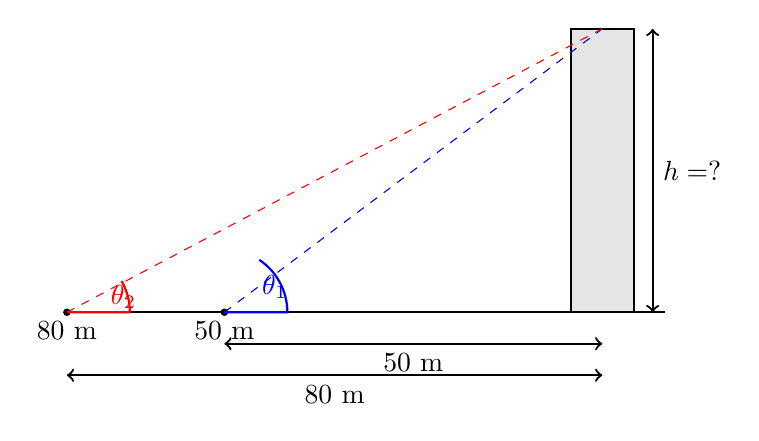
\begin{tikzpicture}[scale=0.8]
    % Suelo
    \draw[thick] (-1,0) -- (8,0);

    % Edificio
    \draw[thick,fill=gray!20] (6.5,0) rectangle (7.5,4.5);

    % Posición inicial del topógrafo
    \draw[fill=black] (1,0) circle (0.05) node[below] {50 m};

    % Línea de visión inicial
    \draw[dashed,blue] (1,0) -- (7,4.5);

    % Ángulo
    \draw[blue,thick] (1,0) -- (2,0) arc[start angle=0, end angle=56.3, radius=1];
    \node[blue] at (1.8,0.4) {$\theta_1$};

    % Posición alejada
    \draw[fill=black] (-1.5,0) circle (0.05) node[below] {80 m};

    % Línea de visión alejada
    \draw[dashed,red] (-1.5,0) -- (7,4.5);

    % Ángulo alejado
    \draw[red,thick] (-1.5,0) -- (-0.5,0) arc[start angle=0, end angle=29.7, radius=1];
    \node[red] at (-0.6,0.25) {$\theta_2$};

    % Altura
    \draw[<->,thick] (7.8,0) -- (7.8,4.5) node[midway,right] {$h = ?$};

    % Distancias
    \draw[<->,thick] (1,-0.5) -- (7,-0.5) node[midway,below] {50 m};
    \draw[<->,thick] (-1.5,-1) -- (7,-1) node[midway,below] {80 m};
\end{tikzpicture}
\end{center}
\end{ejercicio}

\newpage

\section{Soluciones Detalladas}

\begin{solucion}
\textbf{Solución Ejercicio 1:}

Vamos a calcular cada valor recordando que buscamos el ángulo cuya función trigonométrica nos da el valor indicado.

\textbf{a) $\arcsen(0) = ?$}

\textbf{Paso 1:} Debemos encontrar el ángulo $\theta$ tal que $\sen(\theta) = 0$ y $\theta \in [-\pi/2, \pi/2]$.

\textbf{Paso 2:} Sabemos que $\sen(0) = 0$ y $0 \in [-\pi/2, \pi/2]$.

\textbf{Respuesta:} $\arcsen(0) = 0$ radianes

\textbf{b) $\arccos(1) = ?$}

\textbf{Paso 1:} Buscamos $\theta$ tal que $\cos(\theta) = 1$ y $\theta \in [0, \pi]$.

\textbf{Paso 2:} Sabemos que $\cos(0) = 1$ y $0 \in [0, \pi]$.

\textbf{Respuesta:} $\arccos(1) = 0$ radianes

\textbf{c) $\arctan(\sqrt{3}) = ?$}

\textbf{Paso 1:} Necesitamos $\theta$ tal que $\tan(\theta) = \sqrt{3}$ y $\theta \in (-\pi/2, \pi/2)$.

\textbf{Paso 2:} Recordamos que $\tan(\pi/3) = \tan(60°) = \sqrt{3}$ y $\pi/3 \in (-\pi/2, \pi/2)$.

\textbf{Respuesta:} $\arctan(\sqrt{3}) = \frac{\pi}{3}$ radianes

\textbf{d) $\arcsen(-1) = ?$}

\textbf{Paso 1:} Buscamos $\theta$ tal que $\sen(\theta) = -1$ y $\theta \in [-\pi/2, \pi/2]$.

\textbf{Paso 2:} Sabemos que $\sen(-\pi/2) = -1$ y $-\pi/2 \in [-\pi/2, \pi/2]$.

\textbf{Respuesta:} $\arcsen(-1) = -\frac{\pi}{2}$ radianes

\textbf{e) $\arccos(0) = ?$}

\textbf{Paso 1:} Necesitamos $\theta$ tal que $\cos(\theta) = 0$ y $\theta \in [0, \pi]$.

\textbf{Paso 2:} Sabemos que $\cos(\pi/2) = 0$ y $\pi/2 \in [0, \pi]$.

\textbf{Respuesta:} $\arccos(0) = \frac{\pi}{2}$ radianes

\textbf{f) $\arctan(0) = ?$}

\textbf{Paso 1:} Buscamos $\theta$ tal que $\tan(\theta) = 0$ y $\theta \in (-\pi/2, \pi/2)$.

\textbf{Paso 2:} Sabemos que $\tan(0) = 0$ y $0 \in (-\pi/2, \pi/2)$.

\textbf{Respuesta:} $\arctan(0) = 0$ radianes
\end{solucion}

\begin{solucion}
\textbf{Solución Ejercicio 2:}

\textbf{a) $\arccos\left(\frac{\sqrt{2}}{2}\right) = ?$}

\textbf{Paso 1:} Buscamos $\theta$ tal que $\cos(\theta) = \frac{\sqrt{2}}{2}$ y $\theta \in [0, \pi]$.

\textbf{Paso 2:} Recordamos que $\cos(45°) = \cos(\pi/4) = \frac{\sqrt{2}}{2}$ y $\pi/4 \in [0, \pi]$.

\textbf{Respuesta:} $\arccos\left(\frac{\sqrt{2}}{2}\right) = \frac{\pi}{4}$ radianes

\textbf{b) $\arcsen\left(-\frac{1}{2}\right) = ?$}

\textbf{Paso 1:} Necesitamos $\theta$ tal que $\sen(\theta) = -\frac{1}{2}$ y $\theta \in [-\pi/2, \pi/2]$.

\textbf{Paso 2:} Sabemos que $\sen(-30°) = \sen(-\pi/6) = -\frac{1}{2}$ y $-\pi/6 \in [-\pi/2, \pi/2]$.

\textbf{Respuesta:} $\arcsen\left(-\frac{1}{2}\right) = -\frac{\pi}{6}$ radianes

\textbf{c) $\arctan(1) = ?$}

\textbf{Paso 1:} Buscamos $\theta$ tal que $\tan(\theta) = 1$ y $\theta \in (-\pi/2, \pi/2)$.

\textbf{Paso 2:} Recordamos que $\tan(45°) = \tan(\pi/4) = 1$ y $\pi/4 \in (-\pi/2, \pi/2)$.

\textbf{Respuesta:} $\arctan(1) = \frac{\pi}{4}$ radianes

\textbf{d) $\arcsen\left(\frac{\sqrt{3}}{2}\right) = ?$}

\textbf{Paso 1:} Necesitamos $\theta$ tal que $\sen(\theta) = \frac{\sqrt{3}}{2}$ y $\theta \in [-\pi/2, \pi/2]$.

\textbf{Paso 2:} Sabemos que $\sen(60°) = \sen(\pi/3) = \frac{\sqrt{3}}{2}$ y $\pi/3 \in [-\pi/2, \pi/2]$.

\textbf{Respuesta:} $\arcsen\left(\frac{\sqrt{3}}{2}\right) = \frac{\pi}{3}$ radianes

\textbf{e) $\arccos\left(-\frac{1}{2}\right) = ?$}

\textbf{Paso 1:} Buscamos $\theta$ tal que $\cos(\theta) = -\frac{1}{2}$ y $\theta \in [0, \pi]$.

\textbf{Paso 2:} Recordamos que $\cos(120°) = \cos(2\pi/3) = -\frac{1}{2}$ y $2\pi/3 \in [0, \pi]$.

\textbf{Respuesta:} $\arccos\left(-\frac{1}{2}\right) = \frac{2\pi}{3}$ radianes
\end{solucion}

\begin{solucion}
\textbf{Solución Ejercicio 3:}

Para estos ejercicios, usaremos el método del triángulo rectángulo. ¡Es súper útil!

\textbf{a) $\sen\left(\arccos\left(\frac{3}{5}\right)\right) = ?$}

\textbf{Paso 1:} Sea $\theta = \arccos\left(\frac{3}{5}\right)$. Entonces $\cos(\theta) = \frac{3}{5}$.

\textbf{Paso 2:} Dibujamos un triángulo rectángulo donde:
- Cateto adyacente = 3
- Hipotenusa = 5

\begin{center}
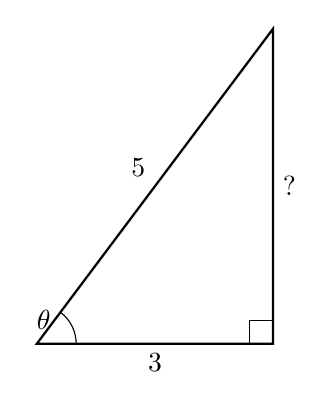
\begin{tikzpicture}[scale=1]
    % Triángulo
    \draw[thick] (0,0) -- (3,0) -- (3,4) -- cycle;
    \draw (2.7,0) -- (2.7,0.3) -- (3,0.3);

    % Etiquetas
    \node[below] at (1.5,0) {3};
    \node[right] at (3,2) {?};
    \node[above left] at (1.5,2) {5};
    \node[left] at (0.3,0.3) {$\theta$};

    % Ángulo
    \draw (0.5,0) arc[start angle=0, end angle=53.13, radius=0.5];
\end{tikzpicture}
\end{center}

\textbf{Paso 3:} Usamos el Teorema de Pitágoras para encontrar el cateto opuesto:
$$\text{opuesto}^2 + 3^2 = 5^2$$
$$\text{opuesto}^2 = 25 - 9 = 16$$
$$\text{opuesto} = 4$$

\textbf{Paso 4:} Por lo tanto:
$$\sen(\theta) = \frac{\text{opuesto}}{\text{hipotenusa}} = \frac{4}{5}$$

\textbf{Respuesta:} $\sen\left(\arccos\left(\frac{3}{5}\right)\right) = \frac{4}{5}$

\textbf{b) $\cos\left(\arcsen\left(\frac{5}{13}\right)\right) = ?$}

\textbf{Paso 1:} Sea $\alpha = \arcsen\left(\frac{5}{13}\right)$. Entonces $\sen(\alpha) = \frac{5}{13}$.

\textbf{Paso 2:} Dibujamos un triángulo rectángulo donde:
- Cateto opuesto = 5
- Hipotenusa = 13

\begin{center}
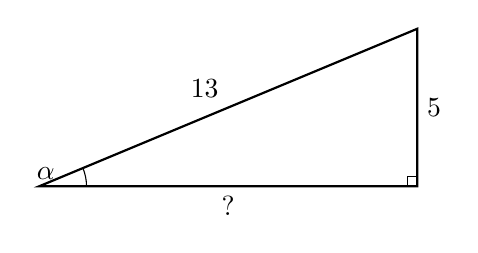
\begin{tikzpicture}[scale=0.4]
    % Triángulo
    \draw[thick] (0,0) -- (12,0) -- (12,5) -- cycle;
    \draw (11.7,0) -- (11.7,0.3) -- (12,0.3);

    % Etiquetas
    \node[below] at (6,0) {?};
    \node[right] at (12,2.5) {5};
    \node[above left] at (6,2.5) {13};
    \node[left] at (0.8,0.4) {$\alpha$};

    % Ángulo
    \draw (1.5,0) arc[start angle=0, end angle=22.62, radius=1.5];
\end{tikzpicture}
\end{center}

\textbf{Paso 3:} Por Pitágoras:
$$\text{adyacente}^2 + 5^2 = 13^2$$
$$\text{adyacente}^2 = 169 - 25 = 144$$
$$\text{adyacente} = 12$$

\textbf{Paso 4:} Entonces:
$$\cos(\alpha) = \frac{\text{adyacente}}{\text{hipotenusa}} = \frac{12}{13}$$

\textbf{Respuesta:} $\cos\left(\arcsen\left(\frac{5}{13}\right)\right) = \frac{12}{13}$

\textbf{c) $\tan\left(\arcsen\left(\frac{2}{3}\right)\right) = ?$}

\textbf{Paso 1:} Sea $\beta = \arcsen\left(\frac{2}{3}\right)$. Entonces $\sen(\beta) = \frac{2}{3}$.

\textbf{Paso 2:} En nuestro triángulo:
- Cateto opuesto = 2
- Hipotenusa = 3

\textbf{Paso 3:} Por Pitágoras:
$$\text{adyacente}^2 + 2^2 = 3^2$$
$$\text{adyacente}^2 = 9 - 4 = 5$$
$$\text{adyacente} = \sqrt{5}$$

\textbf{Paso 4:} La tangente es:
$$\tan(\beta) = \frac{\text{opuesto}}{\text{adyacente}} = \frac{2}{\sqrt{5}} = \frac{2\sqrt{5}}{5}$$

\textbf{Respuesta:} $\tan\left(\arcsen\left(\frac{2}{3}\right)\right) = \frac{2\sqrt{5}}{5}$

\textbf{d) $\sec\left(\arctan\left(\frac{4}{3}\right)\right) = ?$}

\textbf{Paso 1:} Sea $\gamma = \arctan\left(\frac{4}{3}\right)$. Entonces $\tan(\gamma) = \frac{4}{3}$.

\textbf{Paso 2:} En un triángulo rectángulo:
- Cateto opuesto = 4
- Cateto adyacente = 3

\textbf{Paso 3:} Por Pitágoras, la hipotenusa es:
$$\text{hipotenusa}^2 = 4^2 + 3^2 = 16 + 9 = 25$$
$$\text{hipotenusa} = 5$$

\textbf{Paso 4:} Como $\sec(\gamma) = \frac{1}{\cos(\gamma)}$ y $\cos(\gamma) = \frac{3}{5}$:
$$\sec(\gamma) = \frac{5}{3}$$

\textbf{Respuesta:} $\sec\left(\arctan\left(\frac{4}{3}\right)\right) = \frac{5}{3}$
\end{solucion}

\begin{solucion}
\textbf{Solución Ejercicio 4:}

Estas simplificaciones son importantes para entender cómo funcionan las funciones inversas.

\textbf{a) $\sen(\arcsen(x))$ donde $-1 \leq x \leq 1$}

\textbf{Explicación:} Si $\theta = \arcsen(x)$, entonces por definición $\sen(\theta) = x$.

\textbf{Respuesta:} $\sen(\arcsen(x)) = x$ para todo $x \in [-1, 1]$

\textbf{b) $\arcsen(\sen(x))$ para $x \in [-\pi/2, \pi/2]$}

\textbf{Explicación:} Como $x$ ya está en el rango de $\arcsen$, la función arcoseno "deshace" lo que hace el seno.

\textbf{Respuesta:} $\arcsen(\sen(x)) = x$ para $x \in [-\pi/2, \pi/2]$

\textbf{c) $\tan(\arccos(x))$ donde $-1 \leq x \leq 1, x \neq 0$}

\textbf{Paso 1:} Sea $\theta = \arccos(x)$, entonces $\cos(\theta) = x$.

\textbf{Paso 2:} Sabemos que $\sen^2(\theta) + \cos^2(\theta) = 1$, entonces:
$$\sen^2(\theta) = 1 - x^2$$
$$\sen(\theta) = \sqrt{1-x^2}$$ (positivo porque $\theta \in [0,\pi]$)

\textbf{Paso 3:} Por lo tanto:
$$\tan(\theta) = \frac{\sen(\theta)}{\cos(\theta)} = \frac{\sqrt{1-x^2}}{x}$$

\textbf{Respuesta:} $\tan(\arccos(x)) = \frac{\sqrt{1-x^2}}{x}$

\textbf{d) $\cos(\arctan(x))$ para cualquier $x$ real}

\textbf{Paso 1:} Sea $\theta = \arctan(x)$, entonces $\tan(\theta) = x = \frac{x}{1}$.

\textbf{Paso 2:} Podemos pensar en un triángulo rectángulo con:
- Cateto opuesto = $x$ (si $x > 0$) o $|x|$ (si $x < 0$)
- Cateto adyacente = 1
- Hipotenusa = $\sqrt{x^2 + 1}$

\textbf{Paso 3:} Entonces:
$$\cos(\theta) = \frac{\text{adyacente}}{\text{hipotenusa}} = \frac{1}{\sqrt{1+x^2}}$$

\textbf{Respuesta:} $\cos(\arctan(x)) = \frac{1}{\sqrt{1+x^2}}$
\end{solucion}

\begin{solucion}
\textbf{Solución Ejercicio 5:}

\textbf{a) $\arcsen(x) = \frac{\pi}{6}$}

\textbf{Paso 1:} Aplicamos seno a ambos lados:
$$\sen(\arcsen(x)) = \sen\left(\frac{\pi}{6}\right)$$

\textbf{Paso 2:} Simplificamos:
$$x = \frac{1}{2}$$

\textbf{Verificación:} $\arcsen(1/2) = \pi/6$ ✓

\textbf{Respuesta:} $x = \frac{1}{2}$

\textbf{b) $\arccos(2x-1) = \frac{\pi}{3}$}

\textbf{Paso 1:} Aplicamos coseno a ambos lados:
$$\cos(\arccos(2x-1)) = \cos\left(\frac{\pi}{3}\right)$$

\textbf{Paso 2:} Simplificamos:
$$2x - 1 = \frac{1}{2}$$

\textbf{Paso 3:} Resolvemos para $x$:
$$2x = \frac{3}{2}$$
$$x = \frac{3}{4}$$

\textbf{Verificación:} Comprobamos que $2x-1 = 1/2 \in [-1,1]$ ✓

\textbf{Respuesta:} $x = \frac{3}{4}$

\textbf{c) $\arctan(x+1) = \frac{\pi}{4}$}

\textbf{Paso 1:} Aplicamos tangente a ambos lados:
$$\tan(\arctan(x+1)) = \tan\left(\frac{\pi}{4}\right)$$

\textbf{Paso 2:} Simplificamos:
$$x + 1 = 1$$

\textbf{Paso 3:} Resolvemos:
$$x = 0$$

\textbf{Respuesta:} $x = 0$

\textbf{d) $2\arcsen(x) = \frac{\pi}{2}$}

\textbf{Paso 1:} Dividimos entre 2:
$$\arcsen(x) = \frac{\pi}{4}$$

\textbf{Paso 2:} Aplicamos seno:
$$x = \sen\left(\frac{\pi}{4}\right) = \frac{\sqrt{2}}{2}$$

\textbf{Respuesta:} $x = \frac{\sqrt{2}}{2}$

\textbf{e) $\arccos(x) + \arcsen(x) = \frac{\pi}{2}$}

\textbf{Observación:} ¡Esta es una identidad! Es verdadera para todo $x \in [-1,1]$.

\textbf{Demostración rápida:} Si $\theta = \arcsen(x)$, entonces $\sen(\theta) = x$ y $\theta \in [-\pi/2, \pi/2]$.
Como $\cos(\pi/2 - \theta) = \sen(\theta) = x$, tenemos que $\arccos(x) = \pi/2 - \theta = \pi/2 - \arcsen(x)$.

\textbf{Respuesta:} Toda $x \in [-1,1]$ es solución.
\end{solucion}

\begin{solucion}
\textbf{Solución Ejercicio 6:}

\textbf{a) Demostrar: $\arcsen(x) + \arccos(x) = \frac{\pi}{2}$ para $-1 \leq x \leq 1$}

\textbf{Demostración:}

\textbf{Paso 1:} Sea $\alpha = \arcsen(x)$. Por definición, $\sen(\alpha) = x$ y $\alpha \in [-\pi/2, \pi/2]$.

\textbf{Paso 2:} Consideremos el ángulo $\beta = \frac{\pi}{2} - \alpha$. Notemos que:
$$\cos(\beta) = \cos\left(\frac{\pi}{2} - \alpha\right) = \sen(\alpha) = x$$

\textbf{Paso 3:} Además, como $\alpha \in [-\pi/2, \pi/2]$, tenemos que:
$$\beta = \frac{\pi}{2} - \alpha \in [0, \pi]$$

\textbf{Paso 4:} Por la unicidad del arccos en su dominio, $\beta = \arccos(x)$.

\textbf{Paso 5:} Por lo tanto:
$$\arccos(x) = \frac{\pi}{2} - \arcsen(x)$$
$$\arcsen(x) + \arccos(x) = \frac{\pi}{2}$$ ✓

\textbf{b) Demostrar: $\sen(2\arctan(x)) = \frac{2x}{1+x^2}$}

\textbf{Demostración:}

\textbf{Paso 1:} Sea $\theta = \arctan(x)$. Entonces $\tan(\theta) = x$.

\textbf{Paso 2:} En un triángulo rectángulo con $\tan(\theta) = x$:
- Cateto opuesto = $x$ (o $|x|$ si $x < 0$)
- Cateto adyacente = 1
- Hipotenusa = $\sqrt{1+x^2}$

\textbf{Paso 3:} Por lo tanto:
$$\sen(\theta) = \frac{x}{\sqrt{1+x^2}}, \quad \cos(\theta) = \frac{1}{\sqrt{1+x^2}}$$

\textbf{Paso 4:} Usando la fórmula del seno del ángulo doble:
$$\sen(2\theta) = 2\sen(\theta)\cos(\theta)$$
$$= 2 \cdot \frac{x}{\sqrt{1+x^2}} \cdot \frac{1}{\sqrt{1+x^2}}$$
$$= \frac{2x}{1+x^2}$$ ✓

\textbf{c) Demostrar: $\arctan(x) + \arctan\left(\frac{1}{x}\right) = \begin{cases}
\frac{\pi}{2} & \text{si } x > 0 \\
-\frac{\pi}{2} & \text{si } x < 0
\end{cases}$}

\textbf{Demostración para $x > 0$:}

\textbf{Paso 1:} Sean $\alpha = \arctan(x)$ y $\beta = \arctan(1/x)$.

\textbf{Paso 2:} Como $x > 0$, ambos ángulos están en $(0, \pi/2)$.

\textbf{Paso 3:} Notemos que:
$$\tan(\alpha) = x \quad \text{y} \quad \tan(\beta) = \frac{1}{x}$$

\textbf{Paso 4:} Si consideramos $\gamma = \frac{\pi}{2} - \alpha$, entonces:
$$\tan(\gamma) = \tan\left(\frac{\pi}{2} - \alpha\right) = \cot(\alpha) = \frac{1}{\tan(\alpha)} = \frac{1}{x}$$

\textbf{Paso 5:} Como $\gamma \in (0, \pi/2)$ y $\tan(\gamma) = 1/x$, tenemos $\gamma = \beta$.

\textbf{Paso 6:} Por lo tanto:
$$\beta = \frac{\pi}{2} - \alpha$$
$$\alpha + \beta = \frac{\pi}{2}$$ ✓

\textbf{Para $x < 0$:} Un argumento similar muestra que la suma es $-\pi/2$.
\end{solucion}

\begin{solucion}
\textbf{Solución Ejercicio 7 (Problema Aplicado):}

Analicemos este problema de topografía paso a paso.

\textbf{Datos iniciales:}
- Distancia inicial al edificio: 50 metros
- Tangente del ángulo de elevación: $\tan(\theta_1) = \frac{3}{2}$

\textbf{a) ¿Cuál es el ángulo de elevación?}

El ángulo de elevación es:
$$\theta_1 = \arctan\left(\frac{3}{2}\right)$$

En grados: $\theta_1 \approx 56.31°$

\textbf{Respuesta:} El ángulo de elevación es $\arctan(3/2)$ radianes.

\textbf{b) ¿Cuál es la altura del edificio?}

\textbf{Paso 1:} Usando la definición de tangente:
$$\tan(\theta_1) = \frac{\text{altura}}{\text{distancia}} = \frac{h}{50}$$

\textbf{Paso 2:} Como $\tan(\theta_1) = \frac{3}{2}$:
$$\frac{3}{2} = \frac{h}{50}$$

\textbf{Paso 3:} Despejamos $h$:
$$h = 50 \cdot \frac{3}{2} = 75 \text{ metros}$$

\textbf{Respuesta:} La altura del edificio es 75 metros.

\textbf{c) Si el topógrafo se aleja 30 metros más (quedando a 80 metros), ¿cuál será el nuevo ángulo?}

\textbf{Paso 1:} Nueva distancia = 50 + 30 = 80 metros

\textbf{Paso 2:} La tangente del nuevo ángulo es:
$$\tan(\theta_2) = \frac{75}{80} = \frac{15}{16}$$

\textbf{Paso 3:} El nuevo ángulo es:
$$\theta_2 = \arctan\left(\frac{15}{16}\right)$$

En grados: $\theta_2 \approx 43.15°$

\textbf{Respuesta:} El nuevo ángulo de elevación es $\arctan(15/16)$ radianes.

\textbf{d) ¿A qué distancia debe ubicarse para que el ángulo sea de 45°?}

\textbf{Paso 1:} Si el ángulo es 45°, entonces $\tan(45°) = 1$.

\textbf{Paso 2:} Esto significa:
$$\tan(45°) = \frac{75}{d} = 1$$

\textbf{Paso 3:} Despejamos $d$:
$$d = 75 \text{ metros}$$

\textbf{Respuesta:} Debe ubicarse a 75 metros del edificio.

\textbf{Verificación final:}
- A 50 m: $\tan(\theta) = 75/50 = 3/2$ ✓
- A 80 m: $\tan(\theta) = 75/80 = 15/16$ ✓
- A 75 m: $\tan(\theta) = 75/75 = 1$ (ángulo de 45°) ✓

\begin{center}
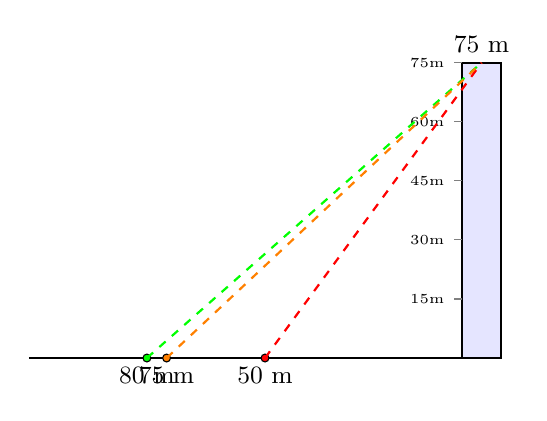
\begin{tikzpicture}[scale=0.05]
    % Suelo
    \draw[thick] (-20,0) -- (100,0);

    % Edificio
    \draw[thick,fill=blue!10] (90,0) rectangle (100,75);

    % Marca de altura
    \foreach \y in {15,30,45,60,75} {
        \draw[gray,thin] (88,\y) -- (90,\y);
        \node[left,font=\tiny] at (88,\y) {\y m};
    }

    % Posiciones del topógrafo
    \draw[fill=red] (40,0) circle (1) node[below] {\small 50 m};
    \draw[fill=green] (10,0) circle (1) node[below] {\small 80 m};
    \draw[fill=orange] (15,0) circle (1) node[below] {\small 75 m};

    % Líneas de visión
    \draw[dashed,red,thick] (40,0) -- (95,75);
    \draw[dashed,green,thick] (10,0) -- (95,75);
    \draw[dashed,orange,thick] (15,0) -- (95,75);

    % Etiqueta del edificio
    \node[above] at (95,75) {\small 75 m};
\end{tikzpicture}
\end{center}

¡Este problema muestra cómo las funciones trigonométricas inversas son súper útiles en la vida real!
\end{solucion}

% Nota final
\begin{nota}
\textbf{¡Felicidades por completar estos ejercicios!}

Recuerda que las funciones trigonométricas inversas son herramientas poderosas que nos permiten "deshacer" las operaciones trigonométricas. Son especialmente útiles en:
\begin{itemize}
    \item Topografía y construcción
    \item Navegación y GPS
    \item Física (análisis de vectores)
    \item Ingeniería y diseño
    \item Computación gráfica y videojuegos
\end{itemize}

¡Sigue practicando y verás que cada vez te resultan más naturales!
\end{nota}